%% Manuscript for Simulation Modelling Practice and Theory (Elsevier), elsarticle class.
%% Every number is a macro generated from the simulation code:
%%   ../paper/generated/*.tex   (paper/make_paper_assets.py)
%%   generated/*.tex            (paper_simpat/make_simpat_assets.py)
\documentclass[preprint,11pt]{elsarticle}

\usepackage[T1]{fontenc}
\usepackage{amsmath,amssymb}
\usepackage{graphicx}
\usepackage{booktabs}
\usepackage{adjustbox}
\usepackage{array}
\usepackage[per-mode=symbol,detect-all]{siunitx}
\usepackage{tikz}
\usetikzlibrary{arrows.meta,positioning}
\usepackage{algorithm}
\usepackage{algpseudocode}
\usepackage{lineno}
\usepackage{xurl}
\usepackage[hidelinks]{hyperref}
\usepackage{setspace}
\linenumbers

\sisetup{range-phrase=--,range-units=single}
\graphicspath{{../paper/figures/}{figures/}}
% Auto-generated by paper/make_paper_assets.py - do not edit by hand.

\newcommand{\YieldL}{1608}
\newcommand{\PRL}{0.819}
\newcommand{\CUFL}{18.35}
\newcommand{\POAL}{1963}
\newcommand{\TdayL}{39.5}
\newcommand{\TmaxL}{57.3}
\newcommand{\TriseL}{10.1}
\newcommand{\RHL}{74.0}
\newcommand{\DewL}{1{,}163}
\newcommand{\SRL}{0.965}
\newcommand{\DegBaseL}{0.30}
\newcommand{\DegTHL}{0.34}
\newcommand{\DegPIDL}{0.15}
\newcommand{\DegCorrL}{0.09}
\newcommand{\DegTotL}{0.88}
\newcommand{\TOWL}{3{,}055}
\newcommand{\RHencL}{63.5}
\newcommand{\LifeL}{36{,}233}
\newcommand{\CapL}{80.9}
\newcommand{\LCOEL}{2.83}
\newcommand{\LossIncidenceAngleL}{3.44}
\newcommand{\LossSpectralL}{-0.23}
\newcommand{\LossSoilingL}{3.67}
\newcommand{\LossDewCondensationL}{0.02}
\newcommand{\LossModuleTemperatureL}{6.12}
\newcommand{\LossDcWiringMismatchMotionLidL}{3.46}
\newcommand{\LossInverterAndClippingL}{2.03}
\newcommand{\LossAvailabilityL}{1.00}
\newcommand{\YieldF}{1634}
\newcommand{\PRF}{0.837}
\newcommand{\CUFF}{18.66}
\newcommand{\POAF}{1953}
\newcommand{\TdayF}{36.5}
\newcommand{\TmaxF}{50.0}
\newcommand{\TriseF}{7.3}
\newcommand{\RHF}{77.5}
\newcommand{\DewF}{1{,}092}
\newcommand{\SRF}{0.988}
\newcommand{\DegBaseF}{0.30}
\newcommand{\DegTHF}{0.34}
\newcommand{\DegPIDF}{0.15}
\newcommand{\DegCorrF}{0.05}
\newcommand{\DegTotF}{0.84}
\newcommand{\TOWF}{3{,}719}
\newcommand{\RHencF}{68.4}
\newcommand{\LifeF}{37{,}004}
\newcommand{\CapF}{81.7}
\newcommand{\LCOEF}{3.54}
\newcommand{\LossIncidenceAngleF}{3.47}
\newcommand{\LossSpectralF}{-0.24}
\newcommand{\LossSoilingF}{1.27}
\newcommand{\LossDewCondensationF}{0.04}
\newcommand{\LossModuleTemperatureF}{4.78}
\newcommand{\LossDcWiringMismatchMotionLidF}{4.62}
\newcommand{\LossInverterAndClippingF}{2.03}
\newcommand{\LossAvailabilityF}{1.50}
\newcommand{\YieldS}{1590}
\newcommand{\PRS}{0.814}
\newcommand{\CUFS}{18.15}
\newcommand{\POAS}{1953}
\newcommand{\TdayS}{36.2}
\newcommand{\TmaxS}{49.4}
\newcommand{\TriseS}{7.0}
\newcommand{\RHS}{79.7}
\newcommand{\DewS}{1{,}389}
\newcommand{\SRS}{0.969}
\newcommand{\DegBaseS}{0.30}
\newcommand{\DegTHS}{0.36}
\newcommand{\DegPIDS}{0.21}
\newcommand{\DegCorrS}{0.30}
\newcommand{\DegTotS}{1.16}
\newcommand{\TOWS}{4{,}288}
\newcommand{\RHencS}{70.4}
\newcommand{\LifeS}{34{,}677}
\newcommand{\CapS}{75.5}
\newcommand{\LCOES}{4.43}
\newcommand{\LossIncidenceAngleS}{3.47}
\newcommand{\LossSpectralS}{-0.25}
\newcommand{\LossSoilingS}{3.29}
\newcommand{\LossDewCondensationS}{0.05}
\newcommand{\LossModuleTemperatureS}{4.64}
\newcommand{\LossDcWiringMismatchMotionLidS}{4.91}
\newcommand{\LossInverterAndClippingS}{2.03}
\newcommand{\LossAvailabilityS}{2.00}
\newcommand{\YieldLM}{1608}
\newcommand{\PRLM}{0.819}
\newcommand{\CUFLM}{18.35}
\newcommand{\POALM}{1963}
\newcommand{\TdayLM}{39.5}
\newcommand{\TmaxLM}{57.3}
\newcommand{\TriseLM}{10.1}
\newcommand{\RHLM}{74.0}
\newcommand{\DewLM}{1{,}163}
\newcommand{\SRLM}{0.965}
\newcommand{\DegBaseLM}{0.30}
\newcommand{\DegTHLM}{0.34}
\newcommand{\DegPIDLM}{0.02}
\newcommand{\DegCorrLM}{0.04}
\newcommand{\DegTotLM}{0.70}
\newcommand{\TOWLM}{3{,}055}
\newcommand{\RHencLM}{63.5}
\newcommand{\LifeLM}{37{,}002}
\newcommand{\CapLM}{84.5}
\newcommand{\LCOELM}{2.90}
\newcommand{\LossIncidenceAngleLM}{3.44}
\newcommand{\LossSpectralLM}{-0.23}
\newcommand{\LossSoilingLM}{3.67}
\newcommand{\LossDewCondensationLM}{0.02}
\newcommand{\LossModuleTemperatureLM}{6.12}
\newcommand{\LossDcWiringMismatchMotionLidLM}{3.46}
\newcommand{\LossInverterAndClippingLM}{2.03}
\newcommand{\LossAvailabilityLM}{1.00}
\newcommand{\YieldFM}{1634}
\newcommand{\PRFM}{0.837}
\newcommand{\CUFFM}{18.66}
\newcommand{\POAFM}{1953}
\newcommand{\TdayFM}{36.5}
\newcommand{\TmaxFM}{50.0}
\newcommand{\TriseFM}{7.3}
\newcommand{\RHFM}{77.5}
\newcommand{\DewFM}{1{,}092}
\newcommand{\SRFM}{0.988}
\newcommand{\DegBaseFM}{0.30}
\newcommand{\DegTHFM}{0.34}
\newcommand{\DegPIDFM}{0.01}
\newcommand{\DegCorrFM}{0.03}
\newcommand{\DegTotFM}{0.68}
\newcommand{\TOWFM}{3{,}719}
\newcommand{\RHencFM}{68.4}
\newcommand{\LifeFM}{37{,}698}
\newcommand{\CapFM}{84.9}
\newcommand{\LCOEFM}{3.60}
\newcommand{\LossIncidenceAngleFM}{3.47}
\newcommand{\LossSpectralFM}{-0.24}
\newcommand{\LossSoilingFM}{1.27}
\newcommand{\LossDewCondensationFM}{0.04}
\newcommand{\LossModuleTemperatureFM}{4.78}
\newcommand{\LossDcWiringMismatchMotionLidFM}{4.62}
\newcommand{\LossInverterAndClippingFM}{2.03}
\newcommand{\LossAvailabilityFM}{1.50}
\newcommand{\YieldSM}{1590}
\newcommand{\PRSM}{0.814}
\newcommand{\CUFSM}{18.15}
\newcommand{\POASM}{1953}
\newcommand{\TdaySM}{36.2}
\newcommand{\TmaxSM}{49.4}
\newcommand{\TriseSM}{7.0}
\newcommand{\RHSM}{79.7}
\newcommand{\DewSM}{1{,}389}
\newcommand{\SRSM}{0.969}
\newcommand{\DegBaseSM}{0.30}
\newcommand{\DegTHSM}{0.36}
\newcommand{\DegPIDSM}{0.02}
\newcommand{\DegCorrSM}{0.15}
\newcommand{\DegTotSM}{0.83}
\newcommand{\TOWSM}{4{,}288}
\newcommand{\RHencSM}{70.4}
\newcommand{\LifeSM}{36{,}045}
\newcommand{\CapSM}{81.9}
\newcommand{\LCOESM}{4.43}
\newcommand{\LossIncidenceAngleSM}{3.47}
\newcommand{\LossSpectralSM}{-0.25}
\newcommand{\LossSoilingSM}{3.29}
\newcommand{\LossDewCondensationSM}{0.05}
\newcommand{\LossModuleTemperatureSM}{4.64}
\newcommand{\LossDcWiringMismatchMotionLidSM}{4.91}
\newcommand{\LossInverterAndClippingSM}{2.03}
\newcommand{\LossAvailabilitySM}{2.00}
\newcommand{\GainYieldF}{1.6}
\newcommand{\GainYieldS}{-1.1}
\newcommand{\GainLifeF}{2.1}
\newcommand{\GainLifeS}{-4.3}
\newcommand{\GainLifeSM}{3.9}
\newcommand{\dTdayF}{3.0}
\newcommand{\dTmaxF}{7.3}
\newcommand{\WaterSaved}{11{,}700}
\newcommand{\GHI}{1{,}889}
\newcommand{\Tair}{28.1}
\newcommand{\RHair}{74.0}
\newcommand{\Rain}{1{,}043}
\newcommand{\SensLifeMin}{32{,}498}
\newcommand{\SensLifeMax}{37{,}005}
\newcommand{\SensDegMin}{0.78}
\newcommand{\SensDegMax}{1.49}
\newcommand{\SensSaltSpan}{2{,}854}
\newcommand{\SensMoistSpan}{1{,}674}
\newcommand{\SensDegPerK}{0.167}
\newcommand{\SensTOWZero}{2{,}253}
\newcommand{\SensTOWMax}{5{,}547}
\newcommand{\SensYieldLoPct}{4.6}
\newcommand{\BreakEvenSalinity}{$<$0.25}
\newcommand{\NSeeds}{20}
\newcommand{\EnsYieldF}{1.71}
\newcommand{\EnsYieldSdF}{0.08}
\newcommand{\EnsLifeF}{2.17}
\newcommand{\EnsLifeSdF}{0.10}
\newcommand{\EnsDegF}{-0.039}
\newcommand{\EnsDegSdF}{0.003}
\newcommand{\EnsYieldS}{-1.08}
\newcommand{\EnsYieldSdS}{0.05}
\newcommand{\EnsLifeS}{-4.32}
\newcommand{\EnsLifeSdS}{0.06}
\newcommand{\EnsDegS}{+0.288}
\newcommand{\EnsDegSdS}{0.002}
\newcommand{\EnsYieldLandMin}{1{,}570}
\newcommand{\EnsYieldLandMax}{1{,}649}
\newcommand{\EnsFreshWins}{20}

% Auto-generated by paper/make_paper_assets.py (review additions) - do not edit by hand.

\newcommand{\NMC}{1{,}000}
\newcommand{\NParams}{28}
\newcommand{\MCYieldMedF}{1.2}
\newcommand{\MCYieldLoF}{$-$1.7}
\newcommand{\MCYieldHiF}{5.3}
\newcommand{\MCYieldPosF}{78}
\newcommand{\MCLifeMedF}{1.5}
\newcommand{\MCLifeLoF}{$-$3.6}
\newcommand{\MCLifeHiF}{6.3}
\newcommand{\MCLifePosF}{75}
\newcommand{\MCYieldMedS}{$-$1.5}
\newcommand{\MCYieldLoS}{$-$5.5}
\newcommand{\MCYieldHiS}{3.1}
\newcommand{\MCYieldPosS}{27}
\newcommand{\MCLifeMedS}{$-$5.1}
\newcommand{\MCLifeLoS}{$-$11.5}
\newcommand{\MCLifeHiS}{0.7}
\newcommand{\MCLifePosS}{4}
\newcommand{\MCYieldMedSM}{$-$1.5}
\newcommand{\MCYieldLoSM}{$-$5.5}
\newcommand{\MCYieldHiSM}{3.1}
\newcommand{\MCYieldPosSM}{27}
\newcommand{\MCLifeMedSM}{$-$1.6}
\newcommand{\MCLifeLoSM}{$-$7.0}
\newcommand{\MCLifeHiSM}{3.8}
\newcommand{\MCLifePosSM}{27}
\newcommand{\RCNameA}{Land dust deposition}
\newcommand{\RCValA}{0.45}
\newcommand{\RCNameB}{FPV $U_1$}
\newcommand{\RCValB}{0.43}
\newcommand{\RCNameC}{Saline salt deposition}
\newcommand{\RCValC}{$-$0.41}
\newcommand{\RCNameD}{FPV $U_0$}
\newcommand{\RCValD}{0.30}
\newcommand{\RCNameE}{Saline chloride deposition}
\newcommand{\RCValE}{$-$0.28}
\newcommand{\RCNameF}{Land $U_1$}
\newcommand{\RCValF}{$-$0.26}
\newcommand{\RCFNameA}{Land dust deposition}
\newcommand{\RCFValA}{0.59}
\newcommand{\RCFNameB}{FPV $U_1$}
\newcommand{\RCFValB}{0.49}
\newcommand{\RCFNameC}{FPV $U_0$}
\newcommand{\RCFValC}{0.35}
\newcommand{\PLcoeF}{99.5}
\newcommand{\PLcoeS}{100.0}
\newcommand{\OATBase}{$-$4.30}
\newcommand{\ClStarText}{none in 0--400}
\newcommand{\SaltStarYield}{35}
\newcommand{\DTdStar}{2.7}
\newcommand{\LifeSalineClZeroPct}{$-$0.9}
\newcommand{\LifeSalineSaltZeroPct}{$-$0.9}
\newcommand{\YieldSalineSaltZeroPct}{1.6}
\newcommand{\DegSalineClMax}{1.31}
\newcommand{\DegSalineClZero}{0.87}
\newcommand{\ClMax}{400}
\newcommand{\TOWFreshAtStar}{5{,}745}
\newcommand{\DewFreshMin}{1.64}
\newcommand{\DewFreshMax}{1.66}
\newcommand{\DewSalineMin}{$-$1.10}
\newcommand{\DewSalineMax}{$-$1.06}
\newcommand{\MitGGvsLand}{1.5}
\newcommand{\MitAllvsLand}{3.3}
\newcommand{\MitPIDRec}{2.2}
\newcommand{\MitSaltRec}{1.7}
\newcommand{\MitBothRec}{3.9}
\newcommand{\MitBothvsLand}{$-$0.5}
\newcommand{\CapexStarF}{34.3}
\newcommand{\CapexStarS}{29.1}
\newcommand{\LandPremF}{10.5}
\newcommand{\LandPremS}{23.6}
\newcommand{\WaterStar}{93}
\newcommand{\LCOEWaterZero}{3.54}
\newcommand{\LCOEWaterTen}{3.47}
\newcommand{\LCOEWaterTwenty}{3.39}
\newcommand{\LCOEWaterForty}{3.24}
\newcommand{\LCOEWaterEighty}{2.93}
\newcommand{\FinGapFMin}{0.58}
\newcommand{\FinGapFMax}{0.86}
\newcommand{\FinGapSMin}{1.36}
\newcommand{\FinGapSMax}{1.87}

\newcommand{\TabMC}{%
Year-1 yield, land (kWh/kWp) & 1{,}604 & [1{,}543, 1{,}638] &  \\
Year-1 yield, FPV fresh (kWh/kWp) & 1{,}624 & [1{,}589, 1{,}645] &  \\
Year-1 yield, FPV saline (kWh/kWp) & 1{,}581 & [1{,}520, 1{,}616] &  \\
Degradation, land (\%/yr) & 0.89 & [0.71, 1.10] &  \\
Degradation, FPV fresh (\%/yr) & 0.88 & [0.68, 1.17] &  \\
Degradation, FPV saline (\%/yr) & 1.21 & [0.91, 1.63] &  \\
Degradation, FPV saline (M) (\%/yr) & 0.91 & [0.67, 1.20] &  \\
$\Delta$ yield, fresh $-$ land (\%) & 1.21 & [$-$1.67, 5.25] & 78 \\
$\Delta$ yield, saline $-$ land (\%) & $-$1.48 & [$-$5.53, 3.06] & 27 \\
$\Delta$ 25-yr energy, fresh $-$ land (\%) & 1.49 & [$-$3.57, 6.33] & 75 \\
$\Delta$ 25-yr energy, saline $-$ land (\%) & $-$5.08 & [$-$11.50, 0.71] & 4 \\
$\Delta$ 25-yr energy, saline (M) $-$ land (\%) & $-$1.56 & [$-$6.96, 3.78] & 27 \\
LCOE, land (INR/kWh) & 2.82 & [2.22, 3.58] &  \\
LCOE, FPV fresh (INR/kWh) & 3.55 & [2.76, 4.55] &  \\
LCOE, FPV saline (INR/kWh) & 4.44 & [3.52, 5.65] &  \\}

\newcommand{\TabMitigation}{%
Standard module & 52.0 & 1.16 & 34{,}677 & 0.0 & $-$4.3 & 4.43 \\
PID-resistant & 52.5 & 0.98 & 35{,}427 & 2.2 & $-$2.2 & 4.41 \\
Salt-mist-hardened & 53.0 & 1.01 & 35{,}277 & 1.7 & $-$2.6 & 4.45 \\
PID + salt-mist & 53.5 & 0.83 & 36{,}045 & 3.9 & $-$0.5 & 4.43 \\
PID + salt-mist + glass-glass & 55.5 & 0.65 & 36{,}792 & 6.1 & 1.5 & 4.50 \\
PID + salt-mist + glass-glass + 7-day cleaning & 55.5 & 0.65 & 37{,}421 & 7.9 & 3.3 & 4.54 \\}

\newcommand{\TabWeather}{%
Mean air temperature (\si{\celsius}) & 28.3 & 28.1 & $-$0.24 & 0.36 & 0.996 \\
Diurnal range (K) & 7.4 & 7.2 & $-$0.20 & 0.23 & 0.993 \\
Mean RH (\%) & 74.0 & 74.0 & 0.00 & 0.00 & 1.000 \\
Mean wind speed (\si{\metre\per\second}) & 3.3 & 3.3 & 0.01 & 0.03 & 0.999 \\
Rainfall (mm)$^{\dagger}$ & 1{,}005.0 & 944.2 & $-$5.07 & 9.71 & 0.995 \\}

\newcommand{\TabFinance}{%
Discount rate 6\% & 2.34 & 2.92 & 3.70 & 0.58 & 1.36 \\
Discount rate 9\% & 2.83 & 3.54 & 4.43 & 0.71 & 1.60 \\
Discount rate 12\% & 3.37 & 4.23 & 5.24 & 0.86 & 1.87 \\
O\&M escalation 2\% & 2.72 & 3.41 & 4.24 & 0.69 & 1.52 \\
O\&M escalation 5\% & 2.83 & 3.54 & 4.43 & 0.71 & 1.60 \\
O\&M escalation 7\% & 2.94 & 3.67 & 4.61 & 0.73 & 1.67 \\}

\newcommand{\TabParams}{%
Peck reference rate $R_{TH}^{ref}$ (\%/yr) & 0.1 & U & 0.06 & 0.14 & Calibration constant; land total $\approx$0.9--1\%/yr~\cite{dubey2014}; $\pm$40\% \\
PID reference rate $R_{PID}^{ref}$ (\%/yr) & 0.06 & U & 0.03 & 0.09 & Calibration constant; $\pm$50\% \\
Corrosion reference rate $R_C^{ref}$ (\%/yr) & 0.1 & U & 0.05 & 0.15 & Calibration constant; $\pm$50\% \\
Dew optical loss & 0.04 & U & 0 & 0.06 & Assumption; effect shown negligible (Sec.~IV-C) \\
Dust loss coefficient $k_d$ (m$^2$/g) & 0.035 & U & 0.025 & 0.045 & Order of magnitude of dust-soiling studies~\cite{sarver2013} \\
Salt loss coefficient $k_s$ (m$^2$/g) & 0.06 & U & 0.03 & 0.09 & Assumption; no measured salt-crust transmittance \\
Deliquescence cementation factor & 0.5 & U & 0.25 & 0.75 & Assumption; salt crusts observed on coastal FPV~\cite{ahmad2026} \\
Land $U_0$ (W/m$^2$K) & 25 & U & 22 & 29 & Around open-rack Faiman defaults~\cite{faiman2008} \\
Land $U_1$ (W\,s/m$^3$K) & 6.84 & U & 4.5 & 8 & Around open-rack Faiman defaults~\cite{faiman2008} \\
Land dust deposition (multiplier) & 1 & log-U & 0.5 & 2 & Assumption; no site measurement \\
Land chloride deposition (multiplier) & 1 & log-U & 0.5 & 2 & 15--60 mg/m$^2$/day, ISO~9223 class S1~\cite{iso9223} \\
FPV $U_0$ (W/m$^2$K) & 35 & U & 22 & 45 & Measured FPV values~\cite{nysted2024,wu2024,dorenkamper2021,lindholm2021} \\
FPV $U_1$ (W\,s/m$^3$K) & 8 & U & 2.5 & 10 & Measured wind terms~\cite{dorenkamper2024,nysted2024} \\
Over-water wind factor $k_v$ & 1.15 & U & 1 & 1.35 & Assumption (lower surface roughness) \\
Wave-motion mismatch & 0.007 & U & 0.003 & 0.015 & Assumption \\
Air--water coupling $\alpha$ (fresh) & 0.25 & U & 0.1 & 0.4 & Assumption \\
Dew-point rise $\Delta T_d$ (fresh, K) & 1 & U & 0.5 & 1.5 & Assumption; threshold analysis in Sec.~IV-F \\
Air--water coupling $\alpha$ (saline) & 0.3 & U & 0.15 & 0.45 & Assumption \\
Dew-point rise $\Delta T_d$ (saline, K) & 1.5 & U & 1 & 2 & Assumption \\
Saline salt deposition (multiplier) & 1 & log-U & 0.5 & 2 & Assumption; threshold analysis in Sec.~IV-F \\
Saline chloride deposition (multiplier) & 1 & log-U & 0.5 & 2 & 90--360 mg/m$^2$/day, ISO~9223 classes S2--S3~\cite{iso9223} \\
PID mitigation $\mu_{PID}$ & 0.9 & U & 0.5 & 0.95 & Assumption (Table~IV); not implied by IEC~TS~62804-1 \\
Salt-mist mitigation $\mu_C$ & 0.5 & U & 0.2 & 0.7 & Assumption (Table~IV); not implied by IEC~61701 \\
Land CAPEX (INR/Wp) & 35 & U & 30 & 40 & Illustrative Indian-market range \\
FPV fresh CAPEX (INR/Wp) & 45 & U & 38 & 52 & Illustrative Indian-market range \\
FPV saline CAPEX (INR/Wp) & 52 & U & 44 & 60 & Illustrative Indian-market range \\
Discount rate & 0.09 & U & 0.06 & 0.12 & Typical range for utility-scale PV finance \\
O\&M escalation & 0.05 & U & 0.02 & 0.07 & Assumption \\}

% Auto-generated: Monte Carlo convergence
\newcommand{\TabConv}{%
$\Delta E_{25}$, fresh & 1.49 (0.09) & 1.42 & [$-$3.57, 6.33] & [$-$3.55, 6.34] \\
$\Delta E_{25}$, saline & $-$5.08 (0.11) & $-$5.12 & [$-$11.50, 0.71] & [$-$11.22, 0.45] \\
$\Delta E_{25}$, saline (M) & $-$1.56 (0.09) & $-$1.65 & [$-$6.96, 3.78] & [$-$7.00, 3.65] \\
$\Delta E_{1}$, fresh & 1.21 (0.07) & 1.11 & [$-$1.67, 5.25] & [$-$1.74, 5.25] \\}
\newcommand{\ConvMaxShift}{0.28}
\newcommand{\ConvMaxSE}{0.30}
\newcommand{\NMCConv}{5{,}000}

% Auto-generated by paper_simpat/make_simpat_assets.py - do not edit by hand.
\newcommand{\PvlibVersion}{0.16.1}
\newcommand{\VerZenMAE}{0.09}
\newcommand{\VerZenMax}{0.25}
\newcommand{\VerAzMAE}{0.24}
\newcommand{\VerPOAEtoE}{0.02}
\newcommand{\VerNExact}{13}
\newcommand{\VerNTotal}{16}
\newcommand{\VerExactMax}{3\times10^{-12}}
\newcommand{\VerErbsMax}{4.2}
\newcommand{\SobolN}{512}
\newcommand{\SobolRuns}{15{,}360}
\newcommand{\SobolEvals}{61{,}440}
\newcommand{\SobFNameA}{Land dust deposition}
\newcommand{\SobFSTA}{0.35}
\newcommand{\SobFNameB}{FPV $U_1$}
\newcommand{\SobFSTB}{0.26}
\newcommand{\SobFNameC}{FPV $U_0$}
\newcommand{\SobFSTC}{0.19}
\newcommand{\SobFSumS}{0.94}
\newcommand{\SobFSumST}{1.04}
\newcommand{\SobFNInfl}{4}
\newcommand{\SobSNameA}{Land dust deposition}
\newcommand{\SobSSTA}{0.22}
\newcommand{\SobSNameB}{FPV $U_1$}
\newcommand{\SobSSTB}{0.21}
\newcommand{\SobSNameC}{Saline salt deposition}
\newcommand{\SobSSTC}{0.17}
\newcommand{\SobSSumS}{0.97}
\newcommand{\SobSSumST}{1.07}
\newcommand{\SobSNInfl}{4}
\newcommand{\RunTimeMs}{23}
\newcommand{\SobolWallMin}{5.1}
\newcommand{\NCores}{4}

\newcommand{\TabVerification}{%
Solar zenith (Spencer vs. SPA) & deg & 4{,}120 & 0.0905 & 0.249 \\
Solar azimuth (Spencer vs. SPA) & deg & 4{,}120 & 0.242 & 1.73 \\
Extraterrestrial irradiance & \% & 8{,}760 & $5.1\times10^{-16}$ & $1.7\times10^{-14}$ \\
Erbs DHI (common solar constant) & W/m$^2$ & 4{,}119 & $4.9\times10^{-14}$ & $2.0\times10^{-12}$ \\
Erbs DNI (common solar constant) & W/m$^2$ & 4{,}119 & $7.3\times10^{-14}$ & $2.6\times10^{-12}$ \\
Erbs DHI (1361 vs. 1366.1 W/m$^2$) & W/m$^2$ & 4{,}119 & 1.81 & 4.19 \\
Hay-Davies sky diffuse & W/m$^2$ & 4{,}119 & $1.6\times10^{-14}$ & $1.1\times10^{-13}$ \\
Angle of incidence & deg & 4{,}119 & $1.5\times10^{-15}$ & $5.2\times10^{-14}$ \\
ASHRAE IAM & -- & 3{,}739 & $3.6\times10^{-18}$ & $6.7\times10^{-16}$ \\
Ground-reflected & W/m$^2$ & 4{,}119 & 0 & 0 \\
Air mass (Kasten-Young) & \% & 4{,}119 & $1.8\times10^{-16}$ & $3.0\times10^{-14}$ \\
Precipitable water (Gueymard) & \% & 8{,}760 & 0 & 0 \\
Spectral factor (First Solar) & -- & 4{,}119 & $3.8\times10^{-19}$ & $2.2\times10^{-16}$ \\
Faiman module temperature & K & 4{,}119 & 0 & 0 \\
PVWatts DC power & kW & 4{,}119 & $1.0\times10^{-14}$ & $2.3\times10^{-13}$ \\
PVWatts inverter & kW & 4{,}119 & 0 & 0 \\}

\newcommand{\TabSobol}{%
Land dust deposition (multiplier) & 0.34 & 0.35$\pm$0.05 & 0.19 & 0.22$\pm$0.03 \\
FPV $U_1$ (W\,s/m$^3$K) & 0.24 & 0.26$\pm$0.04 & 0.20 & 0.21$\pm$0.03 \\
FPV $U_0$ (W/m$^2$K) & 0.16 & 0.19$\pm$0.03 & 0.11 & 0.14$\pm$0.02 \\
Saline salt deposition (multiplier) & 0.00 & 0.00$\pm$0.00 & 0.17 & 0.17$\pm$0.03 \\
Land $U_1$ (W\,s/m$^3$K) & 0.08 & 0.08$\pm$0.01 & 0.05 & 0.05$\pm$0.01 \\
Dust loss coefficient $k_d$ (m$^2$/g) & 0.03 & 0.05$\pm$0.01 & 0.02 & 0.03$\pm$0.01 \\
Salt loss coefficient $k_s$ (m$^2$/g) & 0.00 & 0.00$\pm$0.00 & 0.06 & 0.06$\pm$0.01 \\
Land $U_0$ (W/m$^2$K) & 0.03 & 0.04$\pm$0.01 & 0.02 & 0.02$\pm$0.00 \\
Corrosion reference rate $R_C^{ref}$ (\%/yr) & 0.00 & 0.00$\pm$0.00 & 0.05 & 0.05$\pm$0.01 \\
Saline chloride deposition (multiplier) & 0.00 & 0.00$\pm$0.00 & 0.04 & 0.05$\pm$0.01 \\}


\newcommand{\RHs}{\mathit{RH}_{\mathrm{s}}}
\newcommand{\RHe}{\mathit{RH}_{\mathrm{e}}}
\newcommand{\TOWsym}{\mathit{TOW}}
\newcommand{\yes}{$\checkmark$}

\journal{Simulation Modelling Practice and Theory}

\begin{document}

\begin{frontmatter}

\title{Verified coupled simulation and uncertainty analysis of floating photovoltaic lifetime performance in humid
and saline environments}

\author{Subrahmanyam Tanala\corref{cor1}}
\ead{subrahmanyam.eee@anits.edu.in}
\cortext[cor1]{Corresponding author.}
\affiliation{organization={Department of Electrical and Electronics Engineering, Anil Neerukonda Institute of
Technology and Sciences (ANITS)},
city={Visakhapatnam},
postcode={531162},
state={Andhra Pradesh},
country={India}}

\begin{abstract}
Floating photovoltaic (FPV) plants are expected to outperform land-based plants because water cools the modules, but
the same water raises humidity and, at saline sites, airborne salt, which accelerate soiling and degradation. This
paper presents a simulation framework in which one over-water microclimate drives module temperature, dew, a dust and
sea-salt soiling balance with NaCl deliquescence, and four degradation mechanisms (intrinsic, Peck
temperature--humidity with lagged encapsulant moisture, salt-assisted potential-induced degradation and chloride
corrosion), feeding 25-year energy and levelized cost. The established sub-models are verified code-to-code against
pvlib to within $\VerExactMax$, and every component is classified by its evidential basis. Weather variability and
parameter uncertainty (\NParams{} parameters) are separated using a convergence-checked Monte Carlo and Sobol variance
decomposition. For a hot, humid, coastal site in India, the baseline 25-year energy relative to land PV is
$+\GainLifeF$\% for freshwater and $\GainLifeS$\% for saline FPV. Under parameter uncertainty the freshwater gain is
conditional (median $+$\MCLifeMedF\%, positive in \MCLifePosF\% of samples), whereas the saline penalty is robust
(median \MCLifeMedS\%). Float heat-loss coefficients, land dust load and salt deposition explain most of the variance.
The results are model-based scenario predictions, and a field-validation protocol is proposed.
\end{abstract}

\begin{highlights}
\item Coupled hourly simulation links FPV cooling, humidity, salt soiling, PID, corrosion
\item Sub-models agree with pvlib to 3e-12; Monte Carlo statistics converge at 1,000 runs
\item Freshwater FPV lifetime gain is conditional: positive in 75\% of parameter samples
\item Saline FPV shows a lifetime energy penalty across most of the parameter space
\item Sobol indices rank float heat loss, land dust and salt deposition as key drivers
\end{highlights}

\begin{keyword}
Floating photovoltaics \sep Coupled simulation \sep Verification and validation \sep Uncertainty quantification
\sep Sobol sensitivity analysis \sep Module degradation
\end{keyword}

\end{frontmatter}
\onehalfspacing

%==========================================================================
\section{Introduction}\label{sec:intro}

Floating photovoltaic (FPV) systems place PV arrays on pontoons over reservoirs, lakes, lagoons and sheltered coastal
waters. They avoid competition for land, reduce evaporation from water-supply reservoirs and can share grid
infrastructure with hydropower plants~\cite{worldbank2019,sahu2016,trapani2015,oliveirapinto2020,kumar2021}. Many
candidate sites in South and South-East Asia are hot, humid and exposed to marine aerosol~\cite{makhija2023}. In these
regions, the decision between floating and land-based PV depends on lifetime energy, not on first-year yield alone.

From a modelling perspective, this decision raises three difficulties. First, the mechanisms interact through a shared
microclimate. The water lowers module temperature, which reduces thermal losses and Arrhenius-type
ageing~\cite{liu2018,dorenkamper2021,golroodbari2020}. It also raises humidity, which increases moisture ingress and
PID~\cite{peck1986,kempe2006,hoffmann2014,luo2017}. At saline sites, salt deposits add soiling, lower the surface
resistance of the glass~\cite{hacke2015,islam2018} and drive corrosion~\cite{iso9223}. Simulating each mechanism in
isolation, with independent inputs, cannot resolve these trade-offs. Second, the time scales differ: optical and thermal
processes act hourly, soiling daily, and degradation over decades. Third, many of the governing parameters (heat-loss
coefficients of a given float design, the humidity increment over water, salt and chloride deposition, degradation
reference rates) are uncertain or unmeasured at a candidate site. Measured FPV heat-loss coefficients, for example,
range from values similar to open-rack land PV~\cite{lindholm2021,nysted2024,firat2026} to values much higher for
well-ventilated designs~\cite{dorenkamper2021,wu2024,dorenkamper2024}.

PV simulation practice has addressed parts of this problem. Uncertainty in long-term yield prediction has been
quantified by statistical simulation~\cite{thevenard2013}, and blind intercomparisons show that modelling choices and
derates still cause errors of several percent~\cite{theristis2023,roberts2017}. Climate-dependent degradation models
change lifetime yield estimates substantially compared with fixed rates~\cite{hameed2024,kaaya2019}. Variance-based
sensitivity analysis has been applied to PV degradation in a humid tropical climate~\cite{yuniawan2026}. For offshore
and floating PV, degradation has been forecast from climatic stresses~\cite{mannino2023}, and salinity has been added
to calibrated climatic degradation models~\cite{ajmal2025}. Among the studies reviewed here (Table~\ref{tab:lit}),
none was identified that couples the yield benefits of FPV and its humidity-, salt- and PID-driven penalties within one
microclimate, verifies the implementation, and separates weather from parameter uncertainty with variance-based
sensitivity analysis.

\begin{table}[!t]
\caption{Scope of representative studies (\yes{} = addressed).}
\label{tab:lit}
\centering
\footnotesize
\setlength{\tabcolsep}{3pt}
\begin{adjustbox}{max width=\textwidth}
\begin{tabular}{@{}lccccccccc@{}}
\toprule
Study & FPV & Thermal & Humidity & Salt & PID & Corrosion & Lifetime & UQ & Sobol \\
\midrule
Thevenard and Pelland~\cite{thevenard2013} & & & & & & & \yes & \yes & \\
D{\"o}renk{\"a}mper et al.~\cite{dorenkamper2021} & \yes & \yes & & & & & & & \\
Golroodbari and van Sark~\cite{golroodbari2020} & \yes & \yes & & & & & & & \\
Kaaya et al.~\cite{kaaya2019} & & \yes & \yes & & & & \yes & & \\
Mannino et al.~\cite{mannino2023} & \yes & \yes & \yes & & & & \yes & & \\
Hameed et al.~\cite{hameed2024} & & \yes & \yes & & & & \yes & & \\
Ajmal et al.~\cite{ajmal2025} & \yes & \yes & \yes & \yes & & & \yes & & \\
Ahmad et al.~\cite{ahmad2026} & \yes & \yes & & \yes & & & & & \\
Yuniawan et al.~\cite{yuniawan2026} & & \yes & & & & & \yes & \yes & \yes \\
\textbf{This work} & \yes & \yes & \yes & \yes & \yes & \yes & \yes & \yes & \yes \\
\bottomrule
\end{tabular}
\end{adjustbox}
\end{table}

This paper contributes a simulation framework and its use for a decision problem:
\begin{enumerate}
\item A multi-time-scale coupled model in which one over-water microclimate drives module temperature, dew, spectral
response, soiling and four module-degradation mechanisms (Section~\ref{sec:model}).
\item A verification and validation (V\&V) assessment following established simulation practice~\cite{sargent2013,
oberkampf2010}. It comprises code-to-code verification of the established sub-models against pvlib, a classification of
every component by its evidential basis, a consistency check of the weather generator, and a field-validation protocol
(Section~\ref{sec:vv}).
\item A designed set of simulation experiments that separates weather variability from parameter uncertainty. It
combines a convergence-checked Monte Carlo with Sobol variance decomposition~\cite{sobol2001,saltelli2010} and
break-even analyses (Section~\ref{sec:experiments}).
\item An application to coastal land PV, freshwater FPV and saline FPV in a hot, humid Indian climate, covering energy,
degradation, mitigation and cost (Section~\ref{sec:results}).
\end{enumerate}
The degradation results describe the electrical degradation of the PV modules. Degradation of the floating structure
(float and mooring fatigue, structural corrosion~\cite{xiong2025,feng2025}, storm damage, bio-fouling) is outside the
model.

%==========================================================================
\section{Simulation model}\label{sec:model}

\subsection{Conceptual model and model chain}
Fig.~\ref{fig:chain} shows the model chain. The model is a deterministic, discrete-time simulation with an hourly time
step over one year ($8{,}760$ steps), a daily soiling sub-model, and an annual-rate degradation model extrapolated over
the plant life. Algorithm~\ref{alg:sim} summarizes one scenario evaluation. The established irradiance and electrical
sub-models follow their reference formulations, as implemented in pvlib~\cite{holmgren2018,anderson2023}; they are
re-implemented in vectorized form and verified against pvlib in Section~\ref{sec:vv}.

\begin{figure}[!t]
\centering
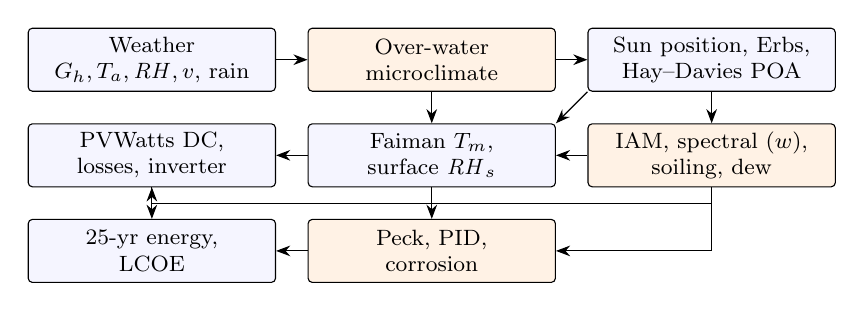
\begin{tikzpicture}[
  font=\footnotesize, node distance=4mm and 4mm,
  box/.style={draw, rounded corners=1.5pt, align=center, minimum height=8mm, inner sep=2pt, text width=30mm,
              fill=blue!4},
  hum/.style={box, fill=orange!10},
  arr/.style={-{Stealth[length=1.8mm]}, thin}]
\node[box] (wx) {Weather\\$G_h, T_a, \mathit{RH}, v$, rain};
\node[hum, right=of wx] (mc) {Over-water\\microclimate};
\node[box, right=of mc] (poa) {Sun position, Erbs,\\Hay--Davies POA};
\node[hum, below=of poa] (opt) {IAM, spectral ($w$),\\soiling, dew};
\node[box, below=of mc] (th) {Faiman $T_m$,\\surface $\mathit{RH}_s$};
\node[box, below=of wx] (el) {PVWatts DC,\\losses, inverter};
\node[hum, below=of th] (deg) {Peck, PID,\\corrosion};
\node[box, below=of el] (life) {25-yr energy,\\LCOE};
\draw[arr] (wx) -- (mc);
\draw[arr] (mc) -- (poa);
\draw[arr] (poa) -- (opt);
\draw[arr] (mc) -- (th);
\draw[arr] (poa.south west) -- (th.north east);
\draw[arr] (opt) -- (th);
\draw[arr] (th) -- (el);
\draw[arr] (opt.south) |- ([yshift=-2mm]th.south) -| (el.south);
\draw[arr] (th) -- (deg);
\draw[arr] (opt.south) |- (deg.east);
\draw[arr] (el) -- (life);
\draw[arr] (deg) -- (life);
\end{tikzpicture}
\caption{Coupled model chain. Shaded blocks depend explicitly on humidity or salinity.}
\label{fig:chain}
\end{figure}

\begin{algorithm}[!t]
\caption{Evaluation of one scenario}
\label{alg:sim}
\begin{algorithmic}[1]
\Require hourly weather $\mathbf{W}$; scenario parameters $\boldsymbol{\theta}$
\State $\mathbf{W}' \gets$ microclimate$(\mathbf{W}; \alpha, \Delta T_d, k_v)$ \Comment{Eq.~\eqref{eq:micro}}
\State sun position, $E_0$; Erbs decomposition; Hay--Davies $G$ \Comment{Eq.~\eqref{eq:poa}}
\For{each day $d$} \Comment{soiling, Eq.~\eqref{eq:soiling}}
  \State add dust and salt; apply rain cleaning (reduced after NaCl deliquescence) and scheduled cleaning
  \State $\mathit{SR}_d \gets \max(\mathit{SR}_{\min}, 1-k_d m_d - k_s m_s)$
\EndFor
\State $T_m \gets$ Faiman$(G, T_a', v')$; $\RHs$; dew state by hysteresis
\State $G_{\mathrm{eff}} \gets G \cdot \mathrm{IAM} \cdot M(\mathit{AM}, w) \cdot \mathit{SR} \cdot (1-\ell_{\mathrm{dew}}\,\mathbb{1}_{\mathrm{wet}})$
\State $P_{\mathrm{ac}} \gets$ inverter$\bigl($PVWatts$(G_{\mathrm{eff}}, T_m)\prod_j(1-\ell_j)\bigr)\cdot$ availability
\State $\RHe \gets$ lag of $\RHs$; evaluate $R_{\mathrm{TH}}, R_{\mathrm{PID}}, R_{\mathrm{C}}$ \Comment{Eqs.~\eqref{eq:rhe}--\eqref{eq:corr}}
\State $R \gets \sum$ mechanisms; $E_y \gets E_1(1-R/100)^{y-1}$; LCOE \Comment{Eq.~\eqref{eq:lcoe}}
\State \Return year-1 losses, $R$ by mechanism, 25-year energy, LCOE
\end{algorithmic}
\end{algorithm}

\subsection{Weather input and over-water microclimate}\label{sec:weather}
The model accepts measured hourly weather. In the absence of a measured series for the reference site, a stochastic
weather generator produces typical years from monthly normals. It draws daily rain occurrence and amounts, a
first-order autoregressive daily clearness index and daily temperature anomalies. Hourly GHI is the Haurwitz clear-sky
value~\cite{haurwitz1945} scaled by the clearness index. Air temperature follows an asymmetric diurnal cycle. The dew
point is held constant over each day and shifted per month so that the monthly mean RH matches the normal. Wind speed
includes a mean-preserving afternoon sea breeze. Over water, the air temperature is pulled towards the water
temperature $T_w$ (30-day running mean of air temperature plus \SI{0.5}{\kelvin}), the dew point rises by $\Delta T_d$,
and the wind speed is scaled:
\begin{equation}
T_a' = T_a + \alpha\,(T_w - T_a),\qquad v' = k_v v,\qquad T_d' = \min(T_d + \Delta T_d,\,T_a').
\label{eq:micro}
\end{equation}
Relative humidity follows from the Magnus relation:
\begin{equation}
\mathit{RH}=100\,\frac{e_s(T_d')}{e_s(T_a')},\qquad e_s(T)=6.112\exp\!\left(\frac{17.62\,T}{243.12+T}\right)~\text{hPa}.
\label{eq:magnus}
\end{equation}

\subsection{Irradiance, incidence and spectrum}
Solar position uses Spencer's series~\cite{spencer1971}. GHI is decomposed with the Erbs correlation~\cite{erbs1982}
and transposed with the Hay--Davies model~\cite{hay1980}:
\begin{equation}
G = G_b\cos\theta + G_d\left[A_i R_b + (1-A_i)\tfrac{1+\cos\beta}{2}\right] + \rho\,G_h\tfrac{1-\cos\beta}{2},
\label{eq:poa}
\end{equation}
where $\theta$ is the angle of incidence, $\beta$ the tilt, $A_i$ the anisotropy index, $R_b$ the beam ratio and $\rho$
the albedo (0.07 for water, 0.20 for land). Beam reflection uses the ASHRAE modifier with $b_0=0.05$. The mono-Si
spectral factor~\cite{lee2016} is computed from the Kasten--Young air mass~\cite{kasten1989} and the precipitable water
$w$~\cite{gueymard1994}:
\begin{equation}
M = c_1 + c_2\mathit{AM} + c_3 w + c_4\sqrt{\mathit{AM}} + c_5\sqrt{w} + c_6\,\mathit{AM}/\sqrt{w}.
\label{eq:spectral}
\end{equation}

\subsection{Module temperature, surface humidity and dew}
Module temperature follows the Faiman model~\cite{faiman2008}, with a net long-wave loss $q_{\mathrm{sky}}=
\SI{40}{\watt\per\square\metre}$ at night:
\begin{equation}
T_m = T_a' + \frac{G - q_{\mathrm{sky}}\,\mathbb{1}[G<50]}{U_0 + U_1 v'}.
\label{eq:faiman}
\end{equation}
The RH of the air in contact with the glass is $\RHs = 100\,e_s(T_d')/e_s(T_m)$, so a hot module is effectively dry and a
module colder than the dew point is wet. Dew forms when $T_m - T_d' < \SI{1}{\kelvin}$ and persists until
$T_m - T_d' > \SI{4}{\kelvin}$. While dew is present, an assumed optical loss of 4\% applies.

\subsection{Dust and sea-salt soiling}
Dust and salt surface densities ($m_d$, $m_s$ in \si{\gram\per\square\metre}) follow a daily mass balance. Dust
accumulates at $r_d$; salt at $r_s v/v_0$ with $v_0=\SI{3}{\metre\per\second}$. Rain above \SI{2}{mm/day} removes a
fraction $\eta f_\beta$ of each deposit ($\eta_d=0.80$, $\eta_s=0.95$, $f_\beta=\sin\beta/\sin\ang{20}$). When the daily
maximum RH exceeds the NaCl deliquescence point of 75\%, the recrystallized salt crust cements dust to the
glass~\cite{ahmad2026}, and the dust-cleaning efficiency is reduced by a cementation factor (0.5). All plants are
cleaned every 15 days. The soiling ratio is
\begin{equation}
\mathit{SR} = \max\left(\mathit{SR}_{\min},\,1 - k_d m_d - k_s m_s\right).
\label{eq:soiling}
\end{equation}
The \emph{salt deposition} $r_s$ is the sea-salt mass retained on the glass. It is distinct from the \emph{chloride
deposition} $D_{\mathrm{Cl}}$ (\si{\milli\gram\per\square\metre\per\day}), the chloride-ion deposition rate of the
atmosphere in the ISO~9223 sense~\cite{iso9223}, which drives corrosion.

\subsection{Electrical model}
DC power follows the PVWatts model~\cite{dobos2014},
$P_{\mathrm{dc}} = P_0 (G_{\mathrm{eff}}/1000)[1+\gamma(T_m-25)]\prod_j(1-\ell_j)$, with $\gamma=\SI{-0.0035}{\per\kelvin}$
and $\ell_j$ the wiring, mismatch, wave-motion and light-induced degradation losses. The PVWatts inverter curve with
clipping and an availability factor follow.

\subsection{Module degradation model}
The annual module degradation rate is the sum of four mechanisms, $R = R_0 + R_{\mathrm{TH}} + R_{\mathrm{PID}} +
R_{\mathrm{C}}$, with $R_0=0.30$\%/yr. Encapsulant moisture follows the surface humidity with a first-order lag
($\tau=\SI{48}{h}$)~\cite{kempe2006}:
\begin{equation}
\RHe(t) = \RHe(t-1) + \kappa\,\bigl[\RHs(t)-\RHe(t-1)\bigr],\qquad \kappa = 1-e^{-\Delta t/\tau}.
\label{eq:rhe}
\end{equation}
With $a_E(T_m)=\exp[-(E/k_B)(1/T_m-1/T_{\mathrm{ref}})]$, the Peck rate~\cite{peck1986} averaged over the year is
\begin{equation}
R_{\mathrm{TH}} = R_{\mathrm{TH}}^{\mathrm{ref}}\left\langle a_{E_a}(T_m)
\left(\frac{\phi\,\RHe}{\mathit{RH}_{\mathrm{ref}}}\right)^{n}\right\rangle,
\label{eq:peck}
\end{equation}
with $E_a=\SI{0.79}{eV}$, $n=3$, $T_{\mathrm{ref}}=\SI{25}{\celsius}$, $\mathit{RH}_{\mathrm{ref}}=60\%$ and $\phi=1$
for glass--backsheet modules. Cooling lowers the Arrhenius factor but raises $\RHe$; \eqref{eq:peck} resolves this
trade-off. PID acts while the array is energized ($G>\SI{50}{\watt\per\square\metre}$):
\begin{equation}
R_{\mathrm{PID}} = R_{\mathrm{PID}}^{\mathrm{ref}}(1-\mu_{\mathrm{PID}})
\bigl\langle a_{E_{\mathrm{PID}}}(T_m)\,f_{\mathrm{leak}}\bigr\rangle_{\mathrm{on}},
\label{eq:pid}
\end{equation}
\begin{equation}
f_{\mathrm{leak}} = \left[1+\exp\left(-\frac{\mathit{RH} - \mathit{RH}_{50}^{*}}{w}\right)\right]^{-1},\qquad
\mathit{RH}_{50}^{*} = \mathit{RH}_{50} - \Delta_s\, s,
\label{eq:leak}
\end{equation}
with $E_{\mathrm{PID}}=\SI{0.9}{eV}$, $\mathit{RH}_{50}=70\%$, width $w=5\%$~RH and threshold shift
$\Delta_s=15\%$~RH. The salt coverage is $s=\min(m_s/0.5,\,1)$ with $m_s$ in \si{\gram\per\square\metre}. The steep humidity dependence of PID leakage~\cite{hoffmann2014,luo2017} and the drop in glass
surface resistance with sea salt~\cite{hacke2015,islam2018} are experimentally supported. The logistic form and its
parameters are modelling choices that have not been fitted to data, so this PID submodel is a physically motivated
scenario model, not a calibrated predictive model. Corrosion uses the ISO~9223 variables~\cite{iso9223}:
\begin{equation}
R_{\mathrm{C}} = R_{\mathrm{C}}^{\mathrm{ref}}\,\frac{\TOWsym}{\TOWsym_{\mathrm{ref}}}
\sqrt{\frac{D_{\mathrm{Cl}}}{D_{\mathrm{ref}}}}\,(1-\mu_{\mathrm{C}}),
\label{eq:corr}
\end{equation}
where $\TOWsym$ counts hours with ambient $\mathit{RH}>80\%$ or dew on the module, $\TOWsym_{\mathrm{ref}}=\SI{2500}{h}$
and $D_{\mathrm{ref}}=\SI{60}{\milli\gram\per\square\metre\per\day}$. This is a calibrated scenario representation, not a
fitted corrosion-damage function. The reference rates ($R_{\mathrm{TH}}^{\mathrm{ref}}=0.10$,
$R_{\mathrm{PID}}^{\mathrm{ref}}=0.06$, $R_{\mathrm{C}}^{\mathrm{ref}}=0.10$\%/yr) were calibrated so that standard
modules on land degrade by roughly 0.9--1\%/yr, the magnitude reported for hot--humid Indian
climates~\cite{dubey2014,jordan2013}.

\subsection{Mitigation options}\label{sec:mit}
Qualification standards define test procedures; they do not establish a numerical reduction of field degradation.
Mitigation therefore enters through explicitly assumed factors (Table~\ref{tab:mitstd}). Salt-mist resistance is
qualified with IEC~61701~\cite{iec61701}, and PID susceptibility with IEC~TS~62804-1~\cite{iec62804}.

\begin{table}[!t]
\caption{Mitigation options: qualification standards and model assumptions. ``(M)'' denotes PID-resistant and
salt-mist-hardened modules. Cost adders: 0.5, 1.0 and 2.0 INR/Wp for the three module options; 100 INR/kWp/yr per
additional fortnightly cleaning.}
\label{tab:mitstd}
\centering
\footnotesize
\begin{adjustbox}{max width=\textwidth}
\begin{tabular}{@{}p{30mm}p{24mm}p{36mm}p{30mm}@{}}
\toprule
Option & Qualification & Model representation & Assumed value (MC range) \\
\midrule
PID-resistant cell/encapsulant & IEC TS 62804-1:2025 & $(1-\mu_{\mathrm{PID}})$ on $R_{\mathrm{PID}}$ & $\mu_{\mathrm{PID}}=0.9$ (0.5--0.95) \\
Salt-mist-hardened module & IEC 61701:2020 & $(1-\mu_{\mathrm{C}})$ on $R_{\mathrm{C}}$ & $\mu_{\mathrm{C}}=0.5$ (0.2--0.7) \\
Glass--glass, low-permeability & No specific standard & Factor $\phi$ on $\RHe$ & $\phi=0.8$ \\
More frequent cleaning & O\&M practice & Cleaning interval & 7 days (vs.\ 15) \\
\bottomrule
\end{tabular}
\end{adjustbox}
\end{table}

\subsection{Lifetime energy and economics}
Year-$y$ energy is $E_y = E_1(1-R/100)^{y-1}$ over $N=25$ years. This assumes a constant effective annual rate derived
from the simulated year's stress distribution. Consequently, the lifetime estimates are equivalent constant-rate
projections, not predictions of the exact annual degradation trajectory. The levelized cost of energy is
\begin{equation}
\mathrm{LCOE} = \frac{C_0 + \sum_{y=1}^{N} (O_y - B_y)(1+r)^{-y}}{\sum_{y=1}^{N}E_y(1+r)^{-y}},
\label{eq:lcoe}
\end{equation}
with discount rate $r=9\%$, O\&M costs $O_y$ escalating by 5\%/yr, and an optional water benefit $B_y=c_wV_w$ for the
evaporation avoided by a freshwater plant (\SI{10}{\square\metre\per\kilo\watt p}, 65\% suppression of
\SI{1800}{mm/yr}). Costs are illustrative Indian-market values, so the economic results are location- and
year-dependent.

\subsection{Implementation and computational cost}
The model is implemented in Python (NumPy, pandas) as an open-source package. All sub-models are vectorized over the
8,760 hours except the three recursive state updates (soiling, dew hysteresis and encapsulant moisture). One scenario-year
takes about \RunTimeMs~ms on one core of the test machine. Monte Carlo and Sobol samples are distributed over
\NCores{} processes. The parameter vectors are drawn in a fixed order, so serial and parallel runs are bit-identical.
The \SobolEvals{} scenario evaluations of the Sobol analysis take about \SobolWallMin~min on \NCores{} cores.

%==========================================================================
\section{Verification and validation}\label{sec:vv}

The V\&V assessment follows the established distinction between conceptual model validity, computerized model
verification, operational validity and data validity~\cite{sargent2013,oberkampf2010}.

\subsection{Conceptual model validity: evidential basis of the components}
Table~\ref{tab:evidence} classifies every model component as an established model used as published (A), a
literature-informed parameter value (B), or a modelling assumption introduced here (C). The contribution lies in the
coupling and in category~C, which is also where field calibration is most needed. Every category-C parameter is varied
in the uncertainty analysis (Appendix~\ref{app:params}).

\begin{table}[!t]
\caption{Evidential basis of the model components.}
\label{tab:evidence}
\centering
\footnotesize
\begin{adjustbox}{max width=\textwidth}
\begin{tabular}{@{}p{6mm}p{124mm}@{}}
\toprule
 & Components \\
\midrule
A & \emph{Established models:} Spencer solar position; Haurwitz clear sky; Erbs decomposition; Hay--Davies
transposition; ASHRAE IAM; Kasten--Young air mass; Gueymard precipitable water; First Solar spectral factor; Magnus
relation; Faiman module temperature; PVWatts DC and inverter models; Arrhenius/Peck functional form; ISO~9223 concepts
of time of wetness and chloride deposition; discounted LCOE. \\
B & \emph{Literature-informed parameters:} land and FPV heat-loss coefficients and their ranges; Peck $E_a$ and $n$;
PID activation energy; NaCl deliquescence RH (75\%); ISO~9223 chloride classes; dust loss coefficient; degradation
reference rates calibrated to the magnitude of Indian field surveys. \\
C & \emph{New modelling assumptions:} over-water microclimate ($\alpha$, $\Delta T_d$, $k_v$, $T_w$); module-surface RH
with a 48-h encapsulant lag; dew criterion and dew optical loss; wind-proportional salt deposition and deliquescence
cementation; salt-assisted logistic leakage function and $\Delta_s$; corrosion scaling $\TOWsym\cdot\sqrt{D_{\mathrm{Cl}}}$;
additive mechanisms with a constant annual rate; mitigation factors and cost adders; all deposition rates and costs. \\
\bottomrule
\end{tabular}
\end{adjustbox}
\end{table}

\subsection{Computerized model verification}
Two techniques are used. First, \emph{code-to-code verification}: each category-A sub-model is compared hour by hour,
over the full baseline year, with the reference implementation in pvlib~\cite{holmgren2018,anderson2023}
(version~\PvlibVersion). Solar position is compared with the NREL solar position algorithm (SPA)~\cite{reda2004}
(Table~\ref{tab:verification}). Of the \VerNTotal{} comparisons, \VerNExact{} agree to within $\VerExactMax$, that is,
to floating-point precision. The Erbs decomposition agrees to the same precision when both codes use the same solar
constant. With the 1361~W/m$^2$ used here instead of pvlib's default of 1366.1~W/m$^2$, the diffuse irradiance differs
by at most \VerErbsMax~W/m$^2$. The only genuine approximation is the Spencer solar-position series. Its mean absolute
zenith error relative to SPA is \VerZenMAE$^\circ$ (maximum \VerZenMax$^\circ$), and it changes the annual
plane-of-array irradiation by \VerPOAEtoE\%, which is negligible for this study.

Second, \emph{unit and regression tests} (23 automated tests) check physical limits and invariants:
\begin{itemize}
\item the noon zenith at the equinox;
\item conservation of GHI in the decomposition;
\item a spectral factor of unity at reference conditions;
\item round-trip consistency of the dew point;
\item PVWatts output at STC and inverter clipping;
\item soiling saturation without cleaning;
\item monotonicity of the degradation rates in temperature, humidity and chloride;
\item reproducibility and serial/parallel equivalence of the Monte Carlo.
\end{itemize}

\begin{table}[!t]
\caption{Code-to-code verification against pvlib \PvlibVersion{} over the baseline year (daytime hours unless stated).
MAE: mean absolute error; Max: maximum absolute error.}
\label{tab:verification}
\centering
\footnotesize
\begin{adjustbox}{max width=\textwidth}
\begin{tabular}{@{}lcccc@{}}
\toprule
Sub-model (this code vs.\ pvlib) & Unit & $n$ & MAE & Max \\
\midrule
\TabVerification
\bottomrule
\end{tabular}
\end{adjustbox}
\end{table}

\subsection{Data validity and the weather generator}
Table~\ref{tab:weather} compares \NSeeds{} generated years with the climatology they are built from. The generator is
climatologically consistent with its inputs; this is a consistency check, not an external validation. The RH match is
exact by construction, and the clearness index (hence GHI) is a calibrated input. The check also served as a
verification step: an earlier version of the generator over-estimated mean wind by about \SI{0.5}{\metre\per\second}
and mean RH by about 2.6 points, and both biases were corrected.

\begin{table}[!t]
\caption{Synthetic-weather consistency check: \NSeeds{} generated years versus the input climatology. MBE, RMSE and
$r$ over the 12 monthly means. $^{\dagger}$Annual totals; MBE and RMSE in mm/month.}
\label{tab:weather}
\centering
\footnotesize
\begin{adjustbox}{max width=\textwidth}
\begin{tabular}{@{}lccccc@{}}
\toprule
Variable & Normal & Generated & MBE & RMSE & $r$ \\
\midrule
\TabWeather
\bottomrule
\end{tabular}
\end{adjustbox}
\end{table}

\subsection{Operational validity: status and protocol}
No measured hourly weather series and no FPV module-temperature, soiling or degradation data were available, so
operational validity could not be established. The results are therefore presented as model-based scenario predictions.
Table~\ref{tab:val} proposes the minimum measurement set for an operating FPV plant with a co-located land reference. It
maps each measurement to the parameters it would calibrate and prioritizes the inputs that the sensitivity analysis
identifies as most influential (Section~\ref{sec:uqres}).

\begin{table}[!t]
\caption{Proposed field-validation measurements and the parameters they calibrate.}
\label{tab:val}
\centering
\footnotesize
\begin{adjustbox}{max width=\textwidth}
\begin{tabular}{@{}p{56mm}p{16mm}p{56mm}@{}}
\toprule
Measurement & Interval & Calibrates \\
\midrule
GHI and POA irradiance (pyranometers) & 1~min & Decomposition, transposition, clearness \\
Air temperature, RH, wind over water and over land & 1~min & $\alpha$, $\Delta T_d$, $k_v$ \\
Water surface temperature & 10~min & $T_w$ \\
Back-of-module temperature (several positions) & 1~min & $U_0$, $U_1$ \\
Dew/leaf-wetness sensor on module glass & 10~min & Dew model, $\TOWsym$ \\
Soiling reference cells (cleaned/uncleaned) & 1~min & $r_d$, $r_s$, $k_d$, $k_s$, cementation \\
Chloride deposition (wet candle, ISO~9225) & Monthly & $D_{\mathrm{Cl}}$ \\
Rainfall; DC power of monitored strings & 1~min & Rain cleaning; PR and loss chain \\
Insulation resistance and leakage current & Daily & $f_{\mathrm{leak}}$, PID onset \\
IV curves of reference modules & Quarterly & $R_{\mathrm{TH}}^{\mathrm{ref}}$, $R_{\mathrm{PID}}^{\mathrm{ref}}$, $R_{\mathrm{C}}^{\mathrm{ref}}$ \\
\bottomrule
\end{tabular}
\end{adjustbox}
\end{table}

%==========================================================================
\section{Design of the simulation experiments}\label{sec:experiments}

\subsection{Case study}
The reference site is Visakhapatnam (\ang{17.69}~N, \ang{83.22}~E) on the Bay of Bengal. Its baseline synthetic year
has a GHI of \GHI~\si{\kilo\watt\hour\per\square\metre}, a mean air temperature of \Tair~\si{\celsius}, a mean RH of
\RHair\% and \Rain~mm of rain (Fig.~\ref{fig:climate}). Three 1-MWp plants (DC/AC ratio 1.2, mono-PERC) are compared
(Table~\ref{tab:params}): coastal land PV; freshwater FPV on an inland reservoir; and saline FPV on near-shore or
brackish water. The baseline values are scenario assumptions.

\begin{figure}[!t]
\centering
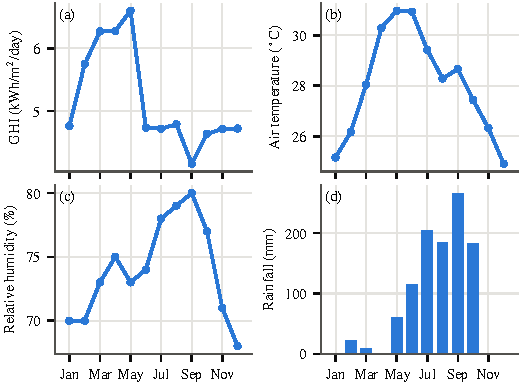
\includegraphics[width=0.62\textwidth]{climate.pdf}
\caption{Monthly climate of the baseline synthetic year: (a) daily GHI, (b) air temperature, (c) relative humidity and
(d) rainfall.}
\label{fig:climate}
\end{figure}

\begin{table}[!t]
\caption{Baseline scenario parameters (assumptions).}
\label{tab:params}
\centering
\footnotesize
\begin{adjustbox}{max width=\textwidth}
\begin{tabular}{@{}lccc@{}}
\toprule
Parameter & Land & FPV fresh & FPV saline \\
\midrule
Tilt (\si{\degree}); albedo & 15; 0.20 & 12; 0.07 & 12; 0.07 \\
$U_0$ (\si{\watt\per\square\metre\per\kelvin}); $U_1$ (\si{\watt\second\per\cubic\metre\per\kelvin}) & 25.0; 6.84 & 35.0; 8.0 & 35.0; 8.0 \\
Air--water coupling $\alpha$; dew-point rise $\Delta T_d$ (K); wind factor $k_v$ & 0; 0; 1.00 & 0.25; 1.0; 1.15 & 0.30; 1.5; 1.25 \\
Dust; salt deposition (\si{\gram\per\square\metre\per\day}) & 0.15; 0.015 & 0.04; 0.010 & 0.03; 0.060 \\
$D_{\mathrm{Cl}}$ (\si{\milli\gram\per\square\metre\per\day}) & 30 & 8 & 180 \\
Wiring loss; wave-motion mismatch; availability (\%) & 1.5; 0; 99.0 & 2.0; 0.7; 98.5 & 2.0; 1.0; 98.0 \\
CAPEX (INR/Wp); O\&M (INR/kWp/yr) & 35; 450 & 45; 550 & 52; 750 \\
\bottomrule
\end{tabular}
\end{adjustbox}
\end{table}

\subsection{Experimental design}
Table~\ref{tab:design} lists the simulation experiments. Two sources of uncertainty are treated separately.
\emph{Weather variability} is represented by \NSeeds{} independent synthetic years (E2). \emph{Parameter uncertainty}
is propagated by Monte Carlo sampling of \NParams{} parameters from uniform or log-uniform distributions (E6). The
parameters, bounds and justifications are listed in Appendix~\ref{app:params}. Parameters shared by the plants take
the same draw within a sample, so scenario differences are paired.

Convergence is assessed by running \NMCConv{} samples with the same seed and evaluating the statistics on nested subsets
of 250--\NMCConv{} samples, with bootstrap standard errors. The first \NMC{} samples are exactly those reported.
Spearman rank correlations screen the parameters. First-order and total-order Sobol indices~\cite{sobol2001} are then
estimated from Saltelli sampling~\cite{saltelli2010} with base sample size $N=\SobolN$, that is $N(D+2)=\SobolRuns$
parameter vectors for $D=\NParams$, using SALib~\cite{herman2017,saltelli2008} (E7). Experiments E3--E5 and E8 are
deterministic sweeps that produce thresholds and break-even values.

\begin{table}[!t]
\caption{Design of the simulation experiments. Each run evaluates the scenarios listed.}
\label{tab:design}
\centering
\footnotesize
\begin{adjustbox}{max width=\textwidth}
\begin{tabular}{@{}p{7mm}p{46mm}p{46mm}p{24mm}@{}}
\toprule
ID & Experiment & Factors varied & Runs \\
\midrule
E1 & Baseline & 3 plants, standard and mitigated modules & 6 \\
E2 & Weather variability & \NSeeds{} weather seeds & $\NSeeds\times3$ \\
E3 & Humidity $\times$ salinity grid (saline) & $\Delta T_d$ (6 levels) $\times$ salt/chloride (5) & 30 \\
E4 & Threshold sweeps & salt (10), chloride (13), $\Delta T_d$ fresh (13) & 36 \\
E5 & Mitigation matrix (saline) & 6 option sets & 6 \\
E6 & Monte Carlo & \NParams{} parameters; \NMC{} (\NMCConv) samples & $4\times$\NMCConv \\
E7 & Sobol decomposition & \NParams{} parameters; $N=\SobolN$ & $4\times$\SobolRuns \\
E8 & Financing sensitivity & discount rate, O\&M escalation & 6 \\
\bottomrule
\end{tabular}
\end{adjustbox}
\end{table}

%==========================================================================
\section{Results}\label{sec:results}

Unless stated otherwise, results are model predictions with the baseline parameters.

\subsection{Thermal behavior and energy yield}
The baseline modelled cooling of the floating modules is \dTdayF~K in daytime, with a peak temperature \dTmaxF~K lower
than on land (Fig.~\ref{fig:temp}, Table~\ref{tab:perf}). This follows from the assumed FPV heat-loss coefficients and is
not a measured effect. At baseline, freshwater FPV has the highest year-1 yield, \YieldF~kWh/kWp ($+\GainYieldF$\%
against land, PR \PRF{} against \PRL). The temperature loss falls from \LossModuleTemperatureL\% to
\LossModuleTemperatureF\% and the soiling loss from \LossSoilingL\% to \LossSoilingF\%. Part of this gain is lost to
higher DC losses, lower availability and slightly lower POA irradiation (Table~\ref{tab:loss}). Salt soiling brings the
saline plant's soiling loss back to \LossSoilingS\%, and its baseline year-1 yield is \YieldS~kWh/kWp
($\GainYieldS$\%). The absolute soiling losses are scenario estimates, because deposition rates were not measured.
Varying the assumed dew optical loss over 0--6\% changes the yield differences by less than 0.05 percentage point.

\begin{figure}[!t]
\centering
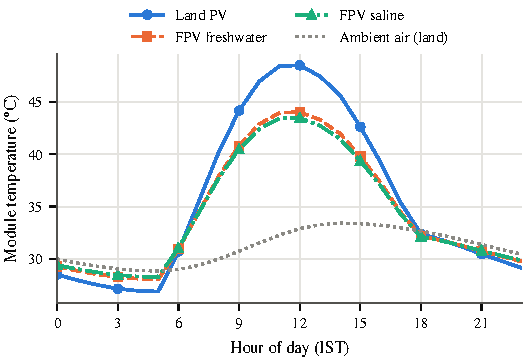
\includegraphics[width=0.62\textwidth]{module_temperature.pdf}
\caption{Mean module temperature by hour of day in May (baseline parameters).}
\label{fig:temp}
\end{figure}

\begin{table}[!t]
\caption{Year-1 performance (baseline).}
\label{tab:perf}
\centering
\footnotesize
\begin{adjustbox}{max width=\textwidth}
\begin{tabular}{@{}lccc@{}}
\toprule
Metric & Land & FPV fresh & FPV saline \\
\midrule
Specific yield (kWh/kWp) & \YieldL & \YieldF & \YieldS \\
Performance ratio & \PRL & \PRF & \PRS \\
Mean daytime / maximum $T_m$ (\si{\celsius}) & \TdayL{} / \TmaxL & \TdayF{} / \TmaxF & \TdayS{} / \TmaxS \\
Mean air RH at array (\%) & \RHL & \RHF & \RHS \\
Dew on glass; time of wetness (h/yr) & \DewL; \TOWL & \DewF; \TOWF & \DewS; \TOWS \\
Mean daytime soiling ratio & \SRL & \SRF & \SRS \\
\bottomrule
\end{tabular}
\end{adjustbox}
\end{table}

\begin{table}[!t]
\caption{Year-1 loss breakdown (baseline). Percentages are sequential losses relative to the preceding stage and are
not directly additive.}
\label{tab:loss}
\centering
\footnotesize
\begin{adjustbox}{max width=\textwidth}
\begin{tabular}{@{}lccc@{}}
\toprule
Loss stage (\%) & Land & FPV fresh & FPV saline \\
\midrule
Incidence angle (IAM) & \LossIncidenceAngleL & \LossIncidenceAngleF & \LossIncidenceAngleS \\
Spectral (humidity) & \LossSpectralL & \LossSpectralF & \LossSpectralS \\
Soiling (dust + salt) & \LossSoilingL & \LossSoilingF & \LossSoilingS \\
Dew / condensation & \LossDewCondensationL & \LossDewCondensationF & \LossDewCondensationS \\
Module temperature & \LossModuleTemperatureL & \LossModuleTemperatureF & \LossModuleTemperatureS \\
DC (wiring, mismatch, motion, LID) & \LossDcWiringMismatchMotionLidL & \LossDcWiringMismatchMotionLidF & \LossDcWiringMismatchMotionLidS \\
Inverter and clipping & \LossInverterAndClippingL & \LossInverterAndClippingF & \LossInverterAndClippingS \\
Availability & \LossAvailabilityL & \LossAvailabilityF & \LossAvailabilityS \\
\bottomrule
\end{tabular}
\end{adjustbox}
\end{table}

\subsection{Module degradation and lifetime energy}\label{sec:dew}
Table~\ref{tab:deg} and Fig.~\ref{fig:deg} resolve the modelled degradation by mechanism. Floating modules are cooler,
but their encapsulant equilibrates at a higher moisture level: mean $\RHe$ is \RHencL\%, \RHencF\% and \RHencS\% at the
three plants. Through the cubic humidity term of \eqref{eq:peck}, this cancels the Arrhenius benefit:
$R_{\mathrm{TH}}$ is \DegTHL, \DegTHF{} and \DegTHS\%/yr. In this model, cooling by water therefore does not translate
into slower moisture-driven ageing at a humid site. PID is highest at the saline plant (\DegPIDS\%/yr), where the salt
film makes the glass conductive at lower RH. Corrosion separates the sites most clearly ($R_{\mathrm{C}}=\DegCorrS$
against \DegCorrL\%/yr). Total degradation is \DegTotL, \DegTotF{} and \DegTotS\%/yr. Over 25 years, the baseline
freshwater plant delivers $+\GainLifeF$\% and the baseline saline plant $\GainLifeS$\% relative to land
(Fig.~\ref{fig:life}).

\begin{figure}[!t]
\centering
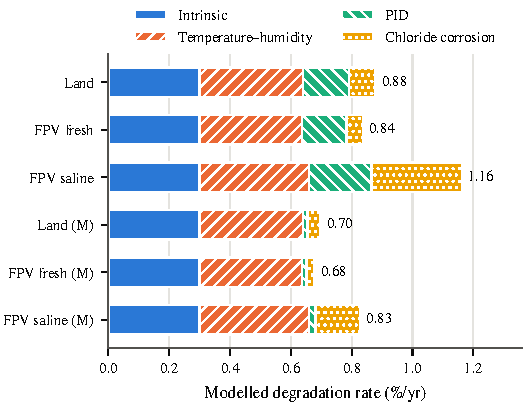
\includegraphics[width=0.62\textwidth]{degradation.pdf}
\caption{Modelled module degradation rate by mechanism (baseline). (M): mitigated modules with the assumed factors of
Table~\ref{tab:mitstd}.}
\label{fig:deg}
\end{figure}

\begin{table}[!t]
\caption{Modelled module degradation, lifetime energy and LCOE (baseline, per MWp).}
\label{tab:deg}
\centering
\footnotesize
\setlength{\tabcolsep}{4pt}
\begin{adjustbox}{max width=\textwidth}
\begin{tabular}{@{}lcccccc@{}}
\toprule
 & Land & FPV fresh & FPV saline & Land (M) & Fresh (M) & Saline (M) \\
\midrule
$R_0$ intrinsic (\%/yr) & \DegBaseL & \DegBaseF & \DegBaseS & \DegBaseLM & \DegBaseFM & \DegBaseSM \\
$R_{\mathrm{TH}}$ (\%/yr) & \DegTHL & \DegTHF & \DegTHS & \DegTHLM & \DegTHFM & \DegTHSM \\
$R_{\mathrm{PID}}$ (\%/yr) & \DegPIDL & \DegPIDF & \DegPIDS & \DegPIDLM & \DegPIDFM & \DegPIDSM \\
$R_{\mathrm{C}}$ (\%/yr) & \DegCorrL & \DegCorrF & \DegCorrS & \DegCorrLM & \DegCorrFM & \DegCorrSM \\
\textbf{Total $R$ (\%/yr)} & \textbf{\DegTotL} & \textbf{\DegTotF} & \textbf{\DegTotS} & \textbf{\DegTotLM} & \textbf{\DegTotFM} & \textbf{\DegTotSM} \\
Mean encapsulant RH (\%) & \RHencL & \RHencF & \RHencS & \RHencLM & \RHencFM & \RHencSM \\
25-year energy (MWh) & \LifeL & \LifeF & \LifeS & \LifeLM & \LifeFM & \LifeSM \\
LCOE (INR/kWh) & \LCOEL & \LCOEF & \LCOES & \LCOELM & \LCOEFM & \LCOESM \\
\bottomrule
\end{tabular}
\end{adjustbox}
\end{table}

\begin{figure}[!t]
\centering
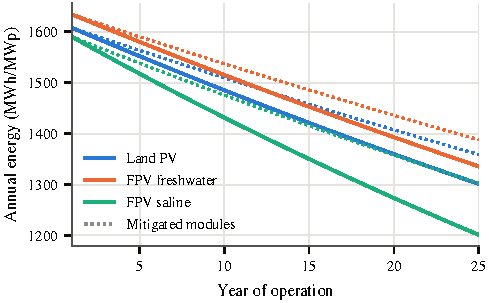
\includegraphics[width=0.62\textwidth]{lifetime.pdf}
\caption{Annual energy over 25 years (baseline). Dotted lines: mitigated modules.}
\label{fig:life}
\end{figure}

\subsection{Thresholds and mitigation}\label{sec:thresholds}
For freshwater FPV, the lifetime advantage over land vanishes at a dew-point rise of $\Delta T_d^*\approx\DTdStar$~K
(Fig.~\ref{fig:thr}b). This is a threshold predicted by the model under the stated assumptions, not a universal
constant, but it can serve as a site-screening criterion. Saline FPV out-yields land in year 1 only below about
\SaltStarYield~\si{\milli\gram\per\square\metre\per\day} of salt deposition. Its 25-year energy stays below land at
every salt level ($\LifeSalineSaltZeroPct$\% at zero salt) and at every chloride level in 0--400
\si{\milli\gram\per\square\metre\per\day} (Fig.~\ref{fig:thr}a). The mitigation matrix (Table~\ref{tab:mitres}) shows
scenario-based, not validated, benefits. PID-resistant and salt-mist-hardened modules together recover \MitBothRec\% of
lifetime energy. Only when a lower-permeability glass--glass package is added does the saline plant exceed land
(\MitGGvsLand\%).

\begin{figure}[!t]
\centering
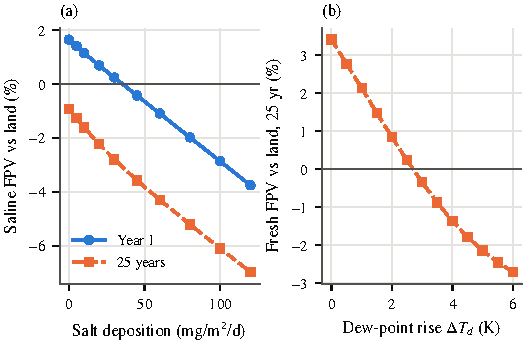
\includegraphics[width=0.62\textwidth]{thresholds.pdf}
\caption{Break-even thresholds relative to land PV. (a) Saline FPV versus salt deposition (chloride at baseline).
(b) Freshwater FPV 25-year energy versus dew-point rise over water.}
\label{fig:thr}
\end{figure}

\begin{table}[!t]
\caption{Scenario-based mitigation benefits for the saline FPV plant (assumed effects of Table~\ref{tab:mitstd}; per
MWp).}
\label{tab:mitres}
\centering
\footnotesize
\setlength{\tabcolsep}{4pt}
\begin{adjustbox}{max width=\textwidth}
\begin{tabular}{@{}lcccccc@{}}
\toprule
Option & CAPEX & $R$ & 25-yr energy & Recovery & vs.\ land & LCOE \\
 & (INR/Wp) & (\%/yr) & (MWh) & (\%) & (\%) & (INR/kWh) \\
\midrule
\TabMitigation
\bottomrule
\end{tabular}
\end{adjustbox}
\end{table}

\subsection{Weather variability, parameter uncertainty and convergence}\label{sec:uqres}
Over \NSeeds{} synthetic years, the yield of the land plant varies between \EnsYieldLandMin{} and
\EnsYieldLandMax~kWh/kWp. The 25-year differences between plants, however, vary with a standard deviation of only about
0.1 percentage point ($+\EnsLifeF\pm\EnsLifeSdF$\% for freshwater and $\EnsLifeS\pm\EnsLifeSdS$\% for saline FPV,
Fig.~\ref{fig:ens}). This is stochastic robustness conditional on the generator, not empirical validation.

Parameter uncertainty is much larger (Table~\ref{tab:mc}, Fig.~\ref{fig:unc}). Baseline values and Monte Carlo medians
answer different questions. For freshwater FPV, the baseline 25-year difference is $+\GainLifeF$\%, whereas the median
is $+$\MCLifeMedF\% with a 95\% interval of [\MCLifeLoF, \MCLifeHiF]\%, positive in \MCLifePosF\% of samples. For saline
FPV, the baseline is $\GainLifeS$\% and the median \MCLifeMedS\% ([\MCLifeLoS, \MCLifeHiS]\%), positive in only
\MCLifePosS\% of samples. The freshwater benefit is therefore conditional, whereas the saline penalty holds across most of
the plausible parameter space. Between \NMC{} and \NMCConv{} samples, no median or 95\% bound moves by more than
\ConvMaxShift~percentage point, and the bootstrap standard errors at \NMC{} samples are at most \ConvMaxSE~percentage point
(Table~\ref{tab:conv}, Fig.~\ref{fig:conv}). \NMC{} samples are therefore sufficient.

\begin{figure}[!t]
\centering
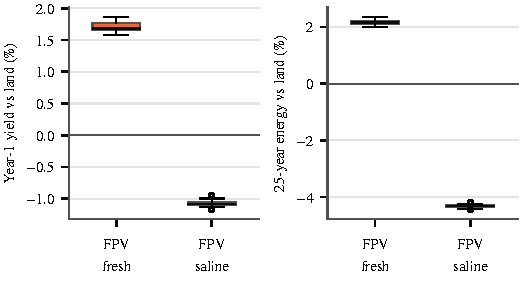
\includegraphics[width=0.62\textwidth]{ensemble.pdf}
\caption{Weather variability only: FPV year-1 yield and 25-year energy relative to land PV over \NSeeds{} synthetic
years.}
\label{fig:ens}
\end{figure}

\begin{table}[!t]
\caption{Parameter uncertainty: Monte Carlo over \NParams{} parameters (\NMC{} samples, baseline weather).}
\label{tab:mc}
\centering
\footnotesize
\begin{adjustbox}{max width=\textwidth}
\begin{tabular}{@{}lccc@{}}
\toprule
Output & Median & 95\% interval & $P(>0)$ (\%) \\
\midrule
\TabMC
\bottomrule
\end{tabular}
\end{adjustbox}
\end{table}

\begin{figure}[!t]
\centering
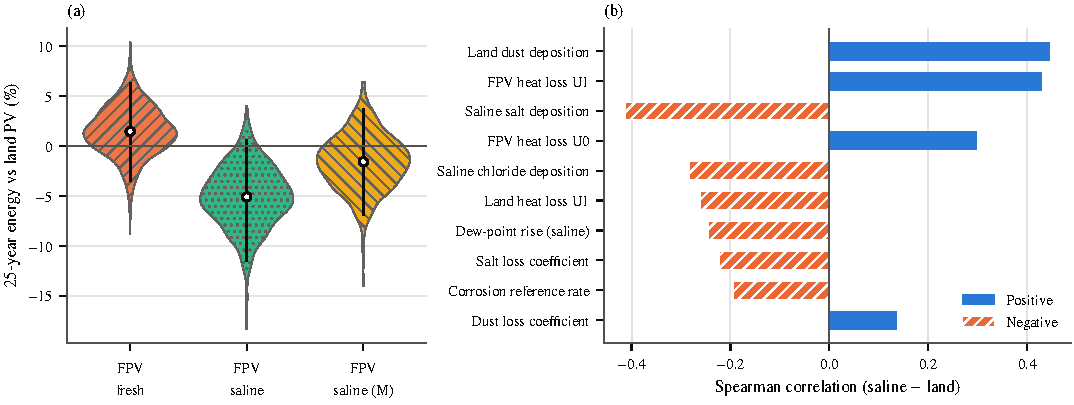
\includegraphics[width=\textwidth]{uncertainty.pdf}
\caption{Parameter uncertainty (\NMC{} samples). (a) 25-year energy relative to land PV (median and 95\% interval).
(b) Spearman rank correlations with the saline minus land difference.}
\label{fig:unc}
\end{figure}

\begin{table}[!t]
\caption{Monte Carlo convergence: \NMC{} versus \NMCConv{} samples. $\Delta E_{25}$ and $\Delta E_1$: 25-year energy and
year-1 yield relative to land PV (\%); bootstrap SE of the median in brackets.}
\label{tab:conv}
\centering
\footnotesize
\begin{adjustbox}{max width=\textwidth}
\begin{tabular}{@{}lcccc@{}}
\toprule
Output & \multicolumn{2}{c}{Median} & \multicolumn{2}{c}{95\% interval} \\
 & $n$=\NMC & $n$=\NMCConv & $n$=\NMC & $n$=\NMCConv \\
\midrule
\TabConv
\bottomrule
\end{tabular}
\end{adjustbox}
\end{table}

\begin{figure}[!t]
\centering
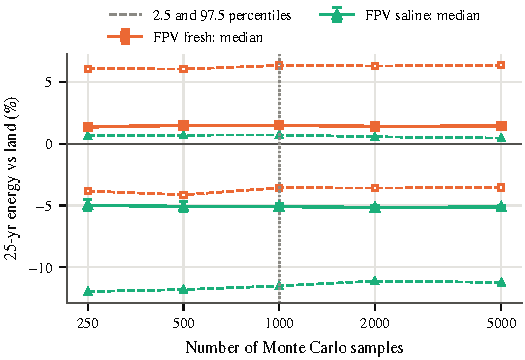
\includegraphics[width=0.62\textwidth]{convergence.pdf}
\caption{Convergence of the Monte Carlo median ($\pm1.96$ bootstrap SE) and 95\% bounds on nested subsets of one
\NMCConv-sample run. The dotted line marks the \NMC{} samples used.}
\label{fig:conv}
\end{figure}

\subsection{Variance-based sensitivity}
Table~\ref{tab:sobol} and Fig.~\ref{fig:sobol} give the Sobol indices of the 25-year energy differences. For freshwater
FPV, \SobFNameA{} ($S_T=\SobFSTA$), \SobFNameB{} (\SobFSTB) and \SobFNameC{} (\SobFSTC) dominate. For saline FPV,
\SobSNameA{} (\SobSSTA), \SobSNameB{} (\SobSSTB) and \SobSNameC{} (\SobSSTC) lead. The first-order indices sum to
\SobFSumS{} and \SobSSumS{}, and the total-order indices to \SobFSumST{} and \SobSSumST. The outputs are therefore close
to additive in the parameters: interactions explain less than about 10\% of the variance. This confirms the
Spearman screening and justifies one-at-a-time threshold analyses. Only \SobFNInfl{} parameters have $S_T$
significantly above 0.05 for each output. Calibrating the float heat-loss coefficients, the dust deposition at the land
alternative and, for saline sites, the salt and chloride deposition would remove most of the decision-relevant
uncertainty.

\begin{figure}[!t]
\centering
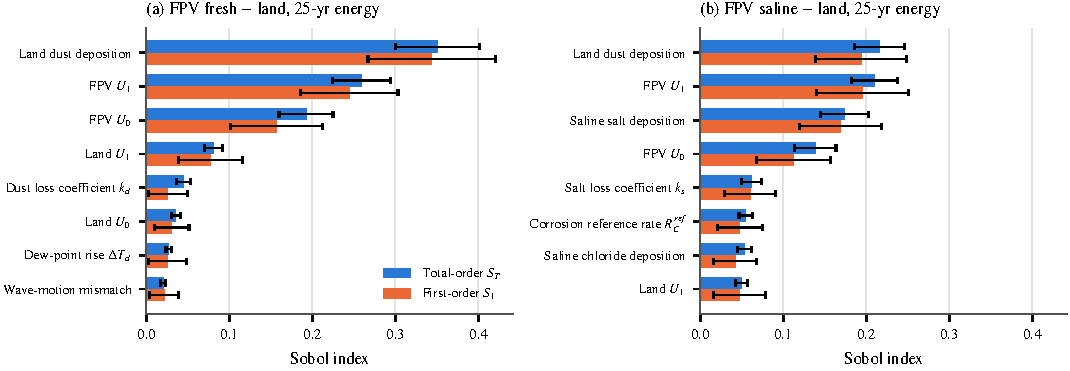
\includegraphics[width=\textwidth]{sobol.pdf}
\caption{First-order and total-order Sobol indices (bootstrap 95\% confidence intervals) of the 25-year energy
difference relative to land PV, for the eight most influential parameters: (a) freshwater FPV, (b) saline FPV.}
\label{fig:sobol}
\end{figure}

\begin{table}[!t]
\caption{Sobol indices of the 25-year energy difference relative to land PV ($N=\SobolN$, $\pm$ bootstrap 95\%
confidence interval), ten most influential parameters.}
\label{tab:sobol}
\centering
\footnotesize
\begin{adjustbox}{max width=\textwidth}
\begin{tabular}{@{}lcccc@{}}
\toprule
 & \multicolumn{2}{c}{FPV fresh $-$ land} & \multicolumn{2}{c}{FPV saline $-$ land} \\
Parameter & $S_1$ & $S_T$ & $S_1$ & $S_T$ \\
\midrule
\TabSobol
\bottomrule
\end{tabular}
\end{adjustbox}
\end{table}

\subsection{Economics}
Under the assumed Indian-market cost and financing conditions, FPV is more expensive per kWh: \LCOEF{} (freshwater) and
\LCOES~INR/kWh (saline), against \LCOEL~INR/kWh on land. This holds in \PLcoeF\% and \PLcoeS\% of Monte Carlo samples.
Parity with land PV requires a CAPEX of \CapexStarF{} (freshwater; baseline 45) or \CapexStarS~INR/Wp (saline;
baseline 52). Alternatively, land PV would need a further \LandPremF{} or \LandPremS~INR/Wp of land-related cost.
Valuing the avoided evaporation (\WaterSaved~m$^3$ per MWp and year) at 10--40~INR/m$^3$ lowers the freshwater LCOE to
\LCOEWaterTen--\LCOEWaterForty~INR/kWh, and parity needs about \WaterStar~INR/m$^3$. Financing assumptions shift all
LCOEs but not their ranking (Table~\ref{tab:fin}).

\begin{table}[!t]
\caption{LCOE sensitivity to financing assumptions (INR/kWh, baseline energy).}
\label{tab:fin}
\centering
\footnotesize
\begin{adjustbox}{max width=\textwidth}
\begin{tabular}{@{}lccccc@{}}
\toprule
Case & Land & FPV fresh & FPV saline & Fresh $-$ land & Saline $-$ land \\
\midrule
\TabFinance
\bottomrule
\end{tabular}
\end{adjustbox}
\end{table}

%==========================================================================
\section{Discussion}\label{sec:discussion}

\subsection{Simulation-methodological lessons}
Three lessons apply beyond this case:
\begin{itemize}
\item \emph{Coupling through a shared state.} The coupling through a shared microclimate and module state is
essential. Evaluating the thermal benefit and the humidity penalty with independent inputs would miss the cancellation
in $R_{\mathrm{TH}}$, because the variable that drives the benefit ($T_m$) also drives the penalty (through $\RHs$).
\item \emph{Separating the sources of uncertainty.} Weather variability alone suggested a precise freshwater advantage
($\pm0.1$ percentage point). Parameter uncertainty showed that this advantage is conditional. Reporting only weather
variability would have overstated the confidence in the result by more than an order of magnitude.
\item \emph{Using the sensitivity analysis to design validation.} The near-additive Sobol structure, with few
influential parameters, means that a compact measurement campaign (Table~\ref{tab:val}) would reduce most of the
decision-relevant uncertainty. Category-C assumptions that turned out to be insensitive, such as the dew optical loss,
need not be measured first.
\end{itemize}

\subsection{Comparison with previous work}
The baseline modelled thermal advantage (about 3~K in daytime, 7~K at peak) lies within the range reported for open,
well-ventilated float designs~\cite{liu2018,dorenkamper2021}. It exceeds that of less ventilated
designs~\cite{nysted2024,firat2026}, which the Monte Carlo covers. The salt-driven increase in degradation is larger than
the 0.05--0.13 percentage-point effect reported for offshore modules~\cite{ajmal2025}. The difference arises because
salt soiling, salt-assisted PID and corrosion are all included here. Consistent with earlier findings that degradation
coefficients must be calibrated to the environment~\cite{mannino2023,hameed2024}, the reference rates used here remain
the main calibration need.

\subsection{Limitations}
\begin{itemize}
\item Operational validity has not been established: no measured weather or FPV data were available.
\item The over-water microclimate, the deposition rates, the degradation reference rates and the mitigation factors are
assumptions. Their uncertainty is propagated, but the ranges themselves are judgements.
\item Degradation is linear in time and additive across mechanisms. PID saturation and recovery, interactions between
mechanisms, abrupt interconnect failures and the higher operating temperature of glass--glass modules are not modelled.
\item Floating-structure degradation is outside the model.
\item The economics are specific to the assumed Indian-market conditions.
\end{itemize}

%==========================================================================
\section{Conclusions}\label{sec:conclusion}
A coupled, multi-time-scale simulation framework for the lifetime performance of floating PV in humid and saline
environments has been developed, verified against the pvlib reference library, and analyzed with separated weather and
parameter uncertainty. For a hot, humid, coastal site in India, the baseline model predicts a modelled cooling of
\dTdayF~K. This gives freshwater FPV a baseline $+\GainYieldF$\% year-1 yield and $+\GainLifeF$\% 25-year energy
relative to land. The humidity increase cancels the temperature benefit for moisture-driven degradation, and at the
saline site salt soiling, salt-assisted PID and chloride corrosion lead to a baseline lifetime deficit of $\GainLifeS$\%.

Under parameter uncertainty, the freshwater benefit is conditional (median $+$\MCLifeMedF\%, positive in \MCLifePosF\% of
samples). In this model it vanishes above a dew-point rise of about \DTdStar~K. The saline penalty is robust (median
\MCLifeMedS\%). Sobol analysis shows near-additive behavior dominated by the float heat-loss coefficients, the dust load
at the land alternative and the salt deposition. These are the quantities a field campaign should measure first.

All results are model-based scenario predictions that require field calibration, for which a measurement protocol is
proposed. The open, verified implementation is intended as a reusable simulation tool for siting and design studies of
floating PV in other humid and saline regions.

%==========================================================================
\section*{CRediT authorship contribution statement}
\textbf{Subrahmanyam Tanala:} Conceptualization, Methodology, Software, Validation, Formal analysis, Investigation,
Visualization, Writing -- original draft, Writing -- review \& editing.

\section*{Declaration of competing interest}
The author declares that there are no known competing financial interests or personal relationships that could have
appeared to influence the work reported in this paper.

\section*{Funding}
This research did not receive any specific grant from funding agencies in the public, commercial, or not-for-profit
sectors.

\section*{Data availability}
The simulation code (\texttt{fpv\_analysis}), its unit tests, all input parameters and Monte Carlo ranges in
machine-readable form, the random seeds, the pinned package versions and every generated table are openly available at
\url{https://github.com/subrahmanyamtanala-rgb/floating-solar-photovoltaic-system-for-humid-and-saline-conditions}. The
command \texttt{./reproduce.sh} regenerates every number, table and figure of this paper.

\section*{Declaration of generative AI and AI-assisted technologies in the manuscript preparation process}
During the preparation of this work the author used Claude (Anthropic) in order to develop the simulation code, run the
simulation experiments, and draft and revise the manuscript text. After using this tool, the author reviewed and edited
the content as needed and takes full responsibility for the content of the published article.

%==========================================================================
\appendix
\setcounter{table}{0}
\section{Monte Carlo parameter space}\label{app:params}
Table~\ref{tab:params_mc} lists the \NParams{} sampled parameters. ``U'' and ``log-U'' denote uniform and log-uniform
distributions; multipliers scale the baseline deposition rates of Table~\ref{tab:params}.

\begin{table}[!t]
\caption{Monte Carlo parameters: baseline, distribution, bounds and justification.}
\label{tab:params_mc}
\centering
\scriptsize
\begin{adjustbox}{max width=\textwidth}
\begin{tabular}{@{}p{42mm}ccccp{48mm}@{}}
\toprule
Parameter & Baseline & Distribution & Lower & Upper & Justification \\
\midrule
\TabParams
\bottomrule
\end{tabular}
\end{adjustbox}
\end{table}

\bibliographystyle{elsarticle-num}
\bibliography{references}

\end{document}
